\chapter{ВЫБОР ТИПА РЕАКТОРА, ПРОТОТИПА И ПАРАМЕТРОВ РЕАКТОРНОЙ
УСТАНОВКИ}

\section{ВВЕДЕНИЕ}

Благодаря атомной энергии человечеству удалось решить ряд важнейших
проблем, связанных с использованием традиционных способов получения
энергии. К ним относятся: борьба за энергоресурсы, увеличение
себестоимости углеводородного топлива, загрязнение окружающей среды и
тд. К тому же, ядерное топливо имеет очень высокую калорийность, по
сравнению с другими видами топлив, к примеру, при выгорании 1г
U\textsuperscript{235} выделяется столько же энергии, сколько в процессе
сжигания 3т высококачественного угля.

В последнее время освоение дальних уголков нашей страны с целью добычи
полезных ископаемых является одним из приоритетных целей и требует
решения ряда энергетических проблем, связанных с затратами на передачу
электроэнергии. Так же нельзя не сказать про судовую ядерную энергетику,
занимающуюся разработкой реакторных установок для боевых надводных и
подводных кораблей военно-морского флота, а так же гражданского атомного
флота, важность которой сложно переоценить. Эти моменты являются
основополагающими в создании реакторных установок малой мощности.

В данной курсовой работе требуется спроектировать ядерную энергетическую
установку (ЯЭУ) малой мощности водо-водяного типа, работающую на
тепловых нейтронах.


\section{Выбор типа реактора}

В России за последние 40 лет АО «ОКБМ им. И.И.Африкантова» было создано
более 360 ядерных реакторов для подводных и надводных кораблей ВМФ и
атомных ледоколов. Особенные требования, предъявляемые к данным судовым
реакторам, сформировали ряд их особенностей -- компактность ЯЭУ, высокая
надежность и уровень безопасности, соответствие требованиям
экологичности \cite{peb}.

ЯЭУ, используемые в судовой ядерной энергетике, делятся на два типа:

\begin{itemize}
\item
  реакторы на быстрых нейтронах, использующий в качестве теплоносителя
  жидкий металл;
\item
  реакторы на тепловых нейтронах -- самая популярная \nom{ЯЭУ}{ядерная энергетическая установка}, использующая
  традиционную для водо-водяных реакторов двухконтурную схему.
\end{itemize}

В упрощенном виде принципиальная тепловая схема судовой ЯЭУ показана на
рис.1.1, она имеет несколько особенностей по сравнению со стационарными
двухконтурными ЯЭУ \cite{xlopkin}:

\begin{enumerate}
\item
  Первый контур должен быть полностью герметичным. Насосы, используемые
  в первом контуре -- бессальниковые; очистка данного контура идет за
  счет прохождения воды через ионообменный фильтр.
\item
  Наличие специального 3\textsuperscript{го} контура для охлаждения
  водой насосных двигателей первого контура, приводов органов
  регулирования, бака металловодной защиты и теплоносителя первого
  контура, идущего на очистку.
\item
  Отсутствие у первого контура арматуры для отключения неисправно
  работающего оборудования.
\item
  Отсутствие предохранительных клапанов в первом контуре. Все
  оборудование имеет высокий запас прочности на случай превышения
  давления; если же давление превосходит максимальное допустимое
  значение, то его нормализация происходит за счет выпускания части
  теплоносителя через специальные фланцевые соединения, которые при
  уменьшении давления сами прекращают сброс воды первого контура.
\end{enumerate}

\begin{figure}[!h]
\center
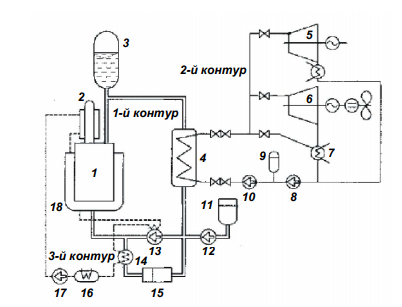
\includegraphics[width=4.56942in,height=3.48958in]{media/image1.png}
\caption{Принципиальная схема ледокольной ЯЭУ: 1-РУ; 2-приводы;
3-компенсатор давления; 4-парогенератор; 5-вспомогательный
турбогенератор; 6-главный турбогенератор; 7-главный конденсатор; 8-
конденсатный насос; 9-уравнительная цистерна; 10-питательный насос;
11-подпиточная система; 12-подпиточный насос; 13-центральный насос
первого контура; 14-холодильник фильтра; 15-ионнообменный фильтр;
16-холодильник 3\textsuperscript{го} контура; 17-циркуляционный насос
3\textsuperscript{го} контура; 18-бак металловодной защиты}
\end{figure}

\section{Выбор прототипа}

В развитии судовых РУ можно выделить 3 поколения судовых ядерных
энергетических установок (табл.1.1)

\begin{quote}
Таблица 1.1 -- Основные характеристики судовых РУ \cite{xlopkin}

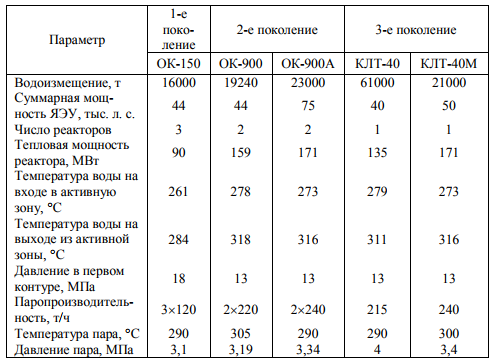
\includegraphics[width=5.59903in,height=4.08333in]{media/image2.png}
\end{quote}

В настоящее время последняя модификация РУ КЛТ-40 -- РУ КЛТ-40С
установлена на строящемся ПЭБ «Академик Ломоносов». Основное отличие РУ
КЛТ-40С от РУ КЛТ-40 -- переход от канальной активной зоны к кассетной.
КЛТ-40С отвечает последним требованиям по безопасности.

\begin{figure}[!h]
\center
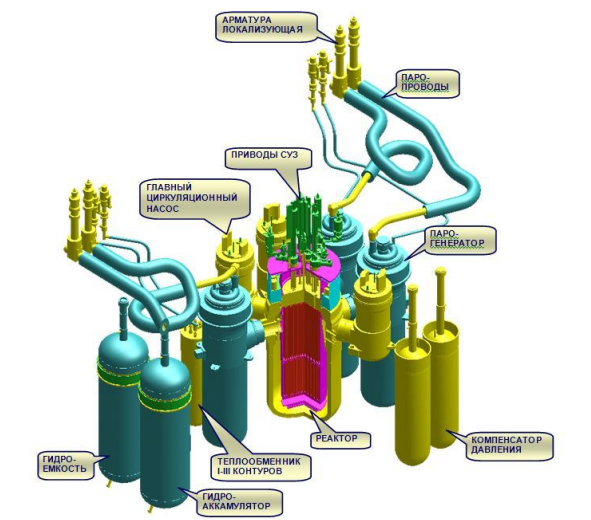
\includegraphics[width=4.56942in,height=3.48958in]{media/image3.png}
\caption{Общий вид РУ КЛТ-40С}
\end{figure}

\section{Анализ прототипа}

Реактор КЛТ-40С -- водо-водяной реактор с двухконтурной системой. Пар
второго контура, поступающий на турбину, изолирован от первого контура и
поэтому не является радиоактивным. Реакторная установка оснащена
надежными «пассивными» системами защиты, функциональность которой
базируется на законах природы - гравитации, конвекции, конденсации.
Благодаря этому, самосрабатывающие устройства системы безопасности не
зависят от электроснабжения.

Наука не стоит на месте, и благодаря этому разрабатываются современные
системы безопасности, внедряются новейшие достижения в области
металловедения, разрабатываются современные электротехнические,
автоматические и микроэлектронные устройства. Именно поэтому РУ КЛТ-40С
отвечает самым высоким требованиям безопасности. Технические
характеристики РУ КЛТ-40С приведены в таблице 1.2 \cite{deev}.

Таблица 1.2 -- Основные технические характеристик РУ КЛТ40-С

\begin{longtable}[]{@{}|l|l|@{}}
\toprule
Параметр, характеристики & Значение\tabularnewline
\midrule
\endhead
Количество РУ в составе энергоблока, шт. & 2\tabularnewline
Температура воды на выходе из реактора, \(\) & 317\tabularnewline
Давление 1-го контура при номинальной мощности, МПа &
12,7\tabularnewline
Температура воды на входе в реактор, \(\) & 294.7\tabularnewline
Энтальпия воды на входе в реактор, Дж/кг & 1439800\tabularnewline
Энтальпия воды на выходе из реактора, Дж/кг & 1311100\tabularnewline
Температура питательной воды, \(\) & 170\tabularnewline
Температура перегретого пара,\(\ \) & 285\tabularnewline
Давление пара за ПГ, МПа & 3.72\tabularnewline
Количество и мощность ЦНПК, кВт & 4х152\tabularnewline
Кампания активной зоны, лет & 2,5-3\tabularnewline
\bottomrule
\end{longtable}

На ПЭБ с РУ КЛТ40-С размещаются две паротурбинные установки
ТК-35/38-3,4. В состав ПТУ входят: паровая турбина, валоповоротное
устройство, система парораспределения, регулирования и защиты. Основные
технические характеристики данной ПТУ представлены в таблице 1.3
\cite{deev}

Таблица 1.3 -- Основные технические характеристик ПТУ ТК-35/38-3,4


\begin{longtable}[]{@{}|l|l|@{}}
\toprule
Наименование параметра & Значение\tabularnewline
\midrule
\endhead
Электрическая мощность, МВт & 35\tabularnewline
Параметры пара перед ПТУ,\(\ \) & 285\tabularnewline
Давление пара перед турбиной, МПа & 3.43\tabularnewline
Температура пара в регулируемом отборе, \(\) & 139.7\tabularnewline
Давление пара в регулируемом отборе, МПа & 0.357\tabularnewline
Давление в конденсаторе, МПа & 0.005\tabularnewline
Расход забортной воды на конденсатор, м\textsuperscript{3}/ч &
5000\tabularnewline
\bottomrule
\end{longtable}

Как уже отмечалось ранее, основное отличие модификации РУ КЛТ-40С от его
предшественника КЛТ-40 состоит в переходе от канальной активной зоны к
кассетной. В таблице 1.4 представлены основные параметры кассетной зоны
реактора КЛТ-40С
\clearpage
Таблица 1.4 -- Основные характеристики кассетной зоны реактора КЛТ-40С

\begin{longtable}[]{@{}|l|l|@{}}
	%\label{Основные характеристики кассетной зоны реактора КЛТ-40С}
\toprule
Параметр & Значение\tabularnewline
\midrule
\endhead
Количество \nom{ТВС}{тепловыделяющая сборка}, шт. & 121\tabularnewline
Диаметр АЗ, мм & 1219\tabularnewline
Высота АЗ H\textsubscript{аз}, мм & 1300\tabularnewline
Диаметр ТВЭЛа, мм & 6,8\tabularnewline
Шаг между ТВЭЛами, мм & 9.6\tabularnewline
Количество ТВЭЛов в АЗ, шт. & 12 342\tabularnewline
Продолжительность кампании, эффективных ч & 22 000\tabularnewline
\bottomrule
\end{longtable}
